\documentclass{article}
% TMLR submission (double-blind): plain \usepackage{tmlr} anonymizes the
% author block and sets the "Under review as submission to TMLR" header.
\usepackage{tmlr}
\usepackage[hyphens]{url}
\usepackage{graphicx}
\usepackage{caption}
\usepackage{booktabs}
\usepackage{multirow}
\usepackage{amsmath}
\usepackage{amssymb}
\frenchspacing
% NOTE: tmlr.sty already loads natbib (and sets authoryear/round citation
% style), so natbib must not be loaded again here.

\title{Diagnosing the CIFAR-10 Gap in Byzantine-Robust, Differentially Private Federated Learning: Evaluation Artifacts and Remaining Limits}

\author{\name Anonymous Author \email anon@example.com \\
        \addr Anonymous Institution}

\begin{document}

\maketitle

\begin{abstract}
Byz-Clip21-SGD2M \citep{islamov2026byzclip} provides high-probability convergence
guarantees for federated learning under simultaneous Byzantine adversaries and
differential-privacy (DP) noise, under a $\sigma$-sub-Gaussian gradient-noise
assumption; its Conclusion lists extending to heavy-tailed noise as future work. In
an earlier stage of this project, stress-testing the algorithm at CIFAR-10 scale
found its accuracy collapses to near-chance under its published protocol, with
CIFAR-10's gradient noise measurably heavier-tailed than MNIST's, and read this as
evidence for a training-difficulty explanation linked to that heavier tail.
Absolute accuracies this low invite an
obvious alternative: that the collapse is a fixable artifact of the evaluation
protocol rather than a property of the algorithm or the dataset. We audit five
candidate explanations -- learning-rate transfer from MNIST, missing
normalization, a miscalibrated clipping ceiling (tested via three
independently-constructed adaptive mechanisms in addition to the published
fixed constant: a quantile tracker, a literature-derived growing schedule, and
an extreme-value-theory-calibrated variant), momentum cold-start, and a missing
clipping floor (tested via a hand-tuned constant and a tail-index-calibrated
variant) -- eight tested mechanisms in total, each inside the unmodified
algorithm, matched to its own published hyperparameters, with paired
significance testing at up to $n{=}10$ seeds. Two of the three clipping-ceiling
mechanisms are ruled out as mechanistically-proven no-ops (the ceiling provably
never binds, confirmed exactly at $n{=}10$, Wilcoxon $p{=}1.000$); the third, an
extreme-value-theory variant designed specifically to avoid that saturation, is
not a proven no-op but empirically shows no effect either (six cells, $n{=}10$,
$p \geq 0.23$). A
four-point learning-rate sweep and a four-point normalization sweep, both now
at $n{=}10$, show no beneficial direction -- retuning the learning rate downward
is significantly \emph{worse} at two of three retuned values (Wilcoxon
$p{=}0.00195$ both, surviving Bonferroni correction across a 21-test family,
the only cells in this audit to do so), and GroupNorm's one nominally-significant
cell does not survive that same correction; momentum cold-start shows a small,
non-significant positive direction at $n{=}10$ ($p \geq 0.43$); and the clipping
floor shows the largest such direction, also non-significant (Wilcoxon
$p{=}0.064$), including when its hand-tuned constant is replaced by a
tail-index-calibrated variant designed specifically to close the gap between
this line of work's own heavy-tail measurements and its clipping hyperparameter
($p \geq 0.275$).
What does close most of the gap is standard machinery absent from the original
protocol: a backbone pretrained centrally on a small, disjoint 10\% public split,
frozen, with a lightweight head federated-trained using the same floor-clipping
mechanism above and more local computation per round -- a disentangling
ablation ($n{=}3$) attributes most of the combined gain to floor-clipping, not
local computation, once applied on top of the pretrained backbone. This raises clean accuracy from
17.1\%$\,\pm\,$3.2\% to 63.1\%$\,\pm\,$0.4\% at matched round budget ($T{=}80$,
$n{=}10$, Wilcoxon $p{=}0.00195$), and to 72.9\%$\,\pm\,$0.1\% with an extended
budget ($T{=}300$), with Byzantine robustness under an omniscient-coalition IPM
attack preserved within 1.4--2.7 percentage points of the clean number -- but
only in the no-DP, IID conditions actually tested. Reintroducing DP noise at
the source algorithm's own privacy budgets collapses this recovery almost
entirely (clean falls to 14--19\%, IPM-attacked accuracy sits within roughly
0.1--0.2 percentage points of the 10\% chance floor at every $\epsilon$
tested, $n{=}3$), and under
non-IID data the clean recovery holds but Byzantine robustness does not (a
roughly 23-percentage-point drop under attack). This configuration resolves
the CIFAR-10 gap in the setting tested, not in the algorithm's actual target
setting of joint Byzantine-robustness and differential privacy under
heterogeneous data -- we report this scope explicitly rather than let the
headline numbers imply otherwise. We report this asymmetry plainly: the fix is
not novel, and we did not find one that is. We also report, as a secondary
finding independent of whether any
resulting algorithm outperforms, a conceptual tension between the two clipping
regimes we tested: the heavy-tailed-noise literature's own convergence guarantees
require a clipping threshold that grows without bound over training, while
Byzantine-robustness guarantees of this algorithm's kind require a threshold that
stays bounded -- a threshold cannot do both at once, which we believe has not
been stated explicitly elsewhere. An attempted comparison against FedProto
\citep{tan2022fedproto}, a structurally unrelated algorithm (it aggregates
class prototypes, not gradients), independently reproduced this paper's central
caution under reduced compute: training collapsed to exactly-chance,
single-class predictions, diagnosed to a representation-collapse failure mode
sensitive to both local computation and client count, not a property of the
algorithm itself; we report the diagnosed failure rather than a number forced
through it. Code, all raw per-seed results, and a written account of two design
iterations that failed and were fixed or reported rather than deleted are
included in the anonymized supplementary material accompanying this
submission, and at \url{https://anonymous.4open.science/r/byzclip-fl-evaluation-artifacts-A4F4/}.
\end{abstract}

\textbf{Keywords.} Byzantine-robust federated learning; differential privacy; evaluation
artifacts; confound analysis; heavy-tailed gradient noise; reproducibility.

\section{Introduction}
\label{sec:intro}

Byz-Clip21-SGD2M \citep{islamov2026byzclip} extends the classical Byzantine-robust
federated learning literature \citep{allouah2023trilemma,karimireddy2020byzantine}
by proving high-probability convergence under \emph{simultaneous} Byzantine
adversaries and differential-privacy noise, relaxing the bounded-gradient
assumption of \citet{allouah2023trilemma} to standard $L$-smoothness and
$\sigma$-sub-Gaussian gradient noise. Its own empirical validation is MNIST-only,
and its Conclusion explicitly lists extending the analysis to heavy-tailed
gradient noise as future work.

This earlier stage of the project stress-tested the algorithm at CIFAR-10 scale
using the harness described in Section~\ref{sec:setup} and found two things.
First, using the established Hill-estimator/kurtosis tail-index methodology of
\citet{simsekli2019tailindex} and follow-ons
\citep{zhang2020adaptive,gurbuzbalaban2021heavytail,barsbey2021compressibility},
CIFAR-10's gradient noise read consistently heavier-tailed than MNIST's across
every statistic and configuration checked (bias-corrected Hill $\alpha \approx
5.4$--$5.9$ for CIFAR-10 versus $\approx 8.0$ for MNIST). Second, CIFAR-10
accuracy under the algorithm's published protocol collapsed to
17.1\%$\,\pm\,$3.2\% ($n{=}10$) even with no Byzantine adversary and no DP noise
active -- a clean, undefended run, on the easier ten-class end of standard image
classification. Reading these two findings together, our most parsimonious
conclusion at that stage was that CIFAR-10's own clean-training convergence
difficulty, plausibly linked to its heavier gradient-noise tail, was the
dominant factor behind the observed gap -- our own earlier conclusion, from the
same authors and codebase, not an external result.

An accuracy this low on a clean, undefended run is also exactly the signature of
a mundane confound: a learning rate transferred from a different dataset without
retuning, a missing normalization layer, a clipping threshold calibrated once and
never revisited, or a momentum mechanism that has not yet warmed up. Before
attributing a collapse this large to an intrinsic property of the noise
distribution, the corresponding protocol-level explanations need to be tested and
ruled out inside the actual algorithm -- not assumed away. This paper is that
audit.

We test five candidate explanations, each holding every other part of the
published protocol fixed and each reporting its own sample size and evidentiary
strength explicitly rather than a uniform standard applied regardless of $n$:
learning-rate transfer (Section~\ref{sec:lr}), missing normalization
(Section~\ref{sec:norm}), a fixed clipping ceiling miscalibrated for a dataset
it was never tuned on and three independently-constructed adaptive alternatives
(Section~\ref{sec:clip}), momentum cold-start
(Section~\ref{sec:momentum}), and a missing clipping floor
(Section~\ref{sec:floor}). The clipping ceiling is ruled out as a
mechanistically-proven no-op; learning-rate transfer and normalization, each
now tested at $n{=}10$, show no beneficial direction in any cell -- retuning
the learning rate downward is significantly worse at two values (surviving
Bonferroni correction, uniquely among every mechanism in this audit), and
normalization's one uncorrected-significant cell does not survive that same
correction; momentum cold-start shows a small, non-significant positive
direction at $n{=}10$; and the clipping floor shows the same direction, more
strongly but still short of significance. None of the five, on the evidence
gathered, is a complete explanation for the collapse. We then
report what does explain most of the gap: standard, non-novel machinery -- a
centrally pretrained, frozen backbone and additional local computation per
communication round -- recovers most of it (Section~\ref{sec:resolution}), and
we are explicit that this is not a new algorithm. Section~\ref{sec:tension}
reports a conceptual byproduct of the audit that survives independently of any
accuracy number: the clipping-threshold behavior that heavy-tailed-noise
convergence theory prescribes and the behavior Byzantine-robustness guarantees
require are in direct tension.

\paragraph{Contributions.} (1) A five-hypothesis, eight-mechanism audit for a
CIFAR-10-scale collapse in a Byzantine-robust, DP-capable federated algorithm,
each hypothesis reported at its own tested sample size and evidentiary
strength rather than a uniform claim: a miscalibrated clipping ceiling ruled
out as a mechanistically-proven no-op; learning-rate transfer and missing
normalization, each tested at $n{=}10$, showing no beneficial direction in any
cell -- retuning the learning rate downward is significantly \emph{worse} at
two values, surviving Bonferroni correction across a 21-test family (the only
cells in this audit to do so), while normalization's one uncorrected-significant
cell does not survive that correction; momentum cold-start showing a small,
non-significant effect at $n{=}10$; and a missing clipping floor's effect real
in direction but not statistically significant. (2) A tail-index-calibrated clipping mechanism, grounded in the
heavy-tailed-SGD literature and this line of work's own tail-index measurements,
designed specifically to close the gap between measurement and algorithm design
-- tested honestly, including a documented first design that failed for a
diagnosable reason, and a corrected second design that also does not
significantly improve accuracy. (3) A demonstration that standard transfer
learning, combined with the same floor-clipping mechanism from (1) and
increased local computation, applied at matched round budgets,
recover most of the apparent gap in the no-DP, IID setting tested, with
Byzantine robustness preserved in that setting -- reported as a resolution of
the confound in the tested conditions, explicitly not as a proposed new
algorithm, and explicitly not shown to extend to DP noise or non-IID data,
where the recovery substantially or entirely fails (Section~\ref{sec:resolution}).
A disentangling ablation (Section~\ref{sec:resolution}, $n{=}3$) further shows
floor-clipping, not local computation, drives most of this additional gain --
the same mechanism that was non-significant in isolation on raw pixels (1),
here roughly 3.5$\times$ larger once combined with the pretrained backbone.
(4) A conceptual observation, independent of (2)'s
empirical outcome, that heavy-tail-optimal and Byzantine-robust clipping
threshold behavior are mutually exclusive over an unbounded time horizon. (5) An
independent, unplanned corroboration of this paper's central caution, found
while attempting a FedProto comparison (Section~\ref{sec:fedproto-attempt}): a
structurally unrelated algorithm exhibits the same exactly-chance,
diagnosable-as-a-training-artifact collapse under reduced compute, reported as
a diagnosed failure mode rather than papered over with a forced number.

\section{Related Work}
\label{sec:related}

\paragraph{Byzantine-robust and DP federated optimization.}
Byz-Clip21-SGD2M \citep{islamov2026byzclip} and its predecessors Safe-DSHB
\citep{allouah2023trilemma} and Byz-Clip-SGD \citep{islamov2026byzclip} combine
robust aggregation
\citep{karimireddy2020byzantine} with per-client gradient clipping and additive
DP noise, and are the algorithms this paper's harness implements and tests
against. \citet{guerraoui2021differential} and \citet{allouah2023trilemma}
characterize the fundamental trade-off between DP noise, Byzantine tolerance, and
utility that motivates clipping-based designs in this setting.

\paragraph{Heavy-tailed gradient noise.} \citet{simsekli2019tailindex} established,
via Hill-estimator tail-index analysis, that SGD gradient noise in deep networks
is empirically heavy-tailed rather than Gaussian; \citet{zhang2020adaptive},
\citet{gurbuzbalaban2021heavytail}, and \citet{barsbey2021compressibility} extend
this measurement methodology to further architectures and consequences. This
paper's tail-index estimator (Section~\ref{sec:clip}) reuses the same class of
statistic, computed online rather than offline.

\paragraph{Clipping under heavy-tailed noise.} \citet{sun2024gradnorm} prove,
under a bounded $p$-th-moment noise model ($p \in (1,2]$, strictly weaker than
bounded variance), that a clipping threshold which \emph{grows} with the round
count is necessary for optimal high-probability convergence, and that gradient
normalization alone suffices for convergence without any clipping under an
individual-Lipschitz condition. This is the direct theoretical source of the
first design of our tail-adaptive clipping mechanism (Section~\ref{sec:clip}),
including the specific way that design fails in our setting.

\paragraph{Adaptive and normalized aggregation.} \citet{andrew2021adaptive}
introduce quantile-tracking adaptive clipping for DP-SGD, estimating the clip
threshold online from the fraction of updates exceeding it; our adaptive-quantile
clipping mechanism (Section~\ref{sec:clip}) adapts this idea to a Byzantine-robust
setting. \citet{zuo2025fedNGA} propose Fed-NGA, aggregating per-client
\emph{normalized} gradients for Byzantine-robust, heterogeneity-tolerant FL; this
is the literature basis for the floor-clipping mechanism in
Section~\ref{sec:clip} and Section~\ref{sec:resolution}'s pretrained-backbone
pipeline.

\paragraph{Federated optimization mechanics.} FedAvg \citep{mcmahan2017fedavg}
introduced multiple local SGD steps per communication round as the mechanism for
trading local computation against communication; \citet{reddi2021adaptive}
formalize a round's resulting client-side model displacement as a server-side
pseudo-gradient, the framing Section~\ref{sec:resolution}'s local-steps mechanism
uses on top of Byz-Clip21-SGD2M's own EF21 double-momentum recursion.

\paragraph{Personalized, model-heterogeneous FL.} FedProto \citep{tan2022fedproto}
aggregates class-prototype embeddings rather than gradients or model weights, for
personalization under model and statistical heterogeneity; its original
formulation includes no Byzantine-robustness or DP mechanism, so it is not a
like-for-like baseline for Byz-Clip21-SGD2M: it targets a different problem
(personalized accuracy under model heterogeneity, evaluated per-client) under a
different threat model (no adversary), and a fair comparison would require
either adding a robustness/privacy mechanism to it or restricting the
comparison to a clean, non-adversarial, non-private setting evaluated on
FedProto's own metric. We attempted a scoped version of the latter anyway
(Section~\ref{sec:fedproto-attempt}) and report what that attempt actually
found -- a training-budget failure mode, not a clean accuracy comparison --
rather than omitting it or forcing a number through it. We note FedProto uses
$T{=}100$/$110$/$120$ rounds for MNIST/CIFAR-10/FEMNIST respectively, 20
clients, and one local epoch per round, which we use in Section~\ref{sec:setup}
as an external reference point for what a standard round budget looks like in
this literature.

\section{Experimental Setup}
\label{sec:setup}

\paragraph{Algorithm and harness.} We use the reference implementation of
Byz-Clip21-SGD2M's Algorithm 1 exactly. Each round: client momentum
$v_i \leftarrow (1-\beta)v_i + \beta \nabla f_i$ tracks client $i$'s gradient
with coefficient $\beta$; a server-side error-feedback state $g_i$ (the "EF21"
mechanism of \citealp{islamov2026byzclip}, itself building on the
communication-compression error-feedback idea) is updated by
$g_i \leftarrow g_i + \hat\beta\,\mathrm{clip}_\tau(v_i-g_i)$ with coefficient
$\hat\beta$, tracking $v_i$ through only the same clipped, bandwidth-limited
signal the server ever receives; each client transmits the clip-then-noise
message $c_i = \mathrm{clip}_\tau(v_i - g_i) + \omega_i$ (Gaussian DP noise
$\omega_i$, zero when $\epsilon{=}\mathrm{None}$); and the server applies
$\mathrm{RAgg}$, a robust aggregator (trimmed mean throughout this paper,
matching the source paper -- discard the largest and smallest few client
values coordinate-wise, then average the rest, so no small minority of
Byzantine clients can dominate the result) to the accumulated state $m_i$.
Unless stated otherwise, every
experiment uses $\beta = \hat\beta = 0.1$, $\gamma = 0.1$ (the source protocol's
own headline step size), $\tau = 1.0$, $n_{\mathrm{regular}}{=}20$ clients, batch
size 32, and IID partitioning via \texttt{partition\_iid}, matching the harness's
existing convention across this line of work.

\paragraph{Datasets and architectures.} MNIST \citep{lecun2010mnist} with a
two-conv-layer CNN (16$\to$32 channels), and CIFAR-10 \citep{krizhevsky2009cifar}
with a two-conv-layer CNN (32$\to$64 channels), both feeding a 64-unit FC layer.
Neither architecture includes batch normalization or data augmentation in the
audited (Sections~\ref{sec:lr}--\ref{sec:floor}) configuration; missing
normalization is itself one of the five candidates audited
(Section~\ref{sec:norm}).

\paragraph{Threat model.} IPM (inner product manipulation) attackers bypass the
honest $v_i/g_i$ pipeline entirely and inject an arbitrary crafted vector
directly into the round's transmitted messages (an omniscient-coalition attack
model, following the source paper); $n_{\mathrm{byzantine}}{=}4$ throughout unless
stated. Label-flip attackers instead follow the honest pipeline exactly but train
on systematically mislabeled data.

\paragraph{Round budget.} The audit (Sections~\ref{sec:lr}--\ref{sec:momentum})
uses $T{=}80$ throughout, matching the source paper's main sweep and close to
FedProto's own CIFAR-10 budget ($T{=}110$; Section~\ref{sec:related}). Where
Section~\ref{sec:resolution} reports results at $T{=}300$, an extended budget
beyond both of these, we state this explicitly rather than blending it silently
into the $T{=}80$ comparison.

\paragraph{Statistical protocol.} Every comparison in this paper is a paired
Wilcoxon signed-rank test (\texttt{scipy.stats.wilcoxon}, two-sided) over matched
seeds, at $n{=}10$ unless explicitly marked as a smaller-$n$ pilot -- and where a
mechanism was only ever run at $n{=}3$, we report it as such rather than implying
a completed scale-up. We define the CONFIRMATORY family as the 21 $p$-values
computed for every mechanism actually tested at $n{=}10$ -- the two floor
mechanisms, clean and IPM; both conditions of the growing-schedule ceiling; the
momentum warm-start, clean and IPM; all six EVT-quantile-ceiling cells; the
three retuned learning rates; and all four GroupNorm cells -- and apply a
Bonferroni correction across that family (family size 21, corrected
$\alpha{=}0.05/21{\approx}0.00238$):
\begin{center}
\small
\begin{tabular}{lc}
\toprule
Test & $p$ \\
\midrule
Hand-tuned floor, clean & 0.105469 \\
Hand-tuned floor, IPM & 0.064453 \\
EVT-quantile floor, clean & 0.275391 \\
EVT-quantile floor, IPM & 0.375000 \\
Growing schedule ceiling, clean & 1.000000 \\
Growing schedule ceiling, IPM & 0.687500 \\
Momentum warm-start, clean & 0.447266 \\
Momentum warm-start, IPM & 0.431641 \\
EVT-quantile ceiling, $q{=}0.01$ clean & 0.814453 \\
EVT-quantile ceiling, $q{=}0.01$ IPM & 0.371094 \\
EVT-quantile ceiling, $q{=}0.05$ clean & 0.570312 \\
EVT-quantile ceiling, $q{=}0.05$ IPM & 0.232422 \\
EVT-quantile ceiling, $q{=}0.2$ clean & 0.671875 \\
EVT-quantile ceiling, $q{=}0.2$ IPM & 0.572266 \\
Learning-rate retune, $\gamma{=}0.05$ & 0.048828 \\
Learning-rate retune, $\gamma{=}0.02$ & 0.001953 \\
Learning-rate retune, $\gamma{=}0.01$ & 0.001953 \\
GroupNorm, $\gamma{=}0.1$ & 0.037109 \\
GroupNorm, $\gamma{=}0.05$ & 0.130859 \\
GroupNorm, $\gamma{=}0.02$ & 0.845703 \\
GroupNorm, $\gamma{=}0.01$ & 0.130859 \\
\bottomrule
\end{tabular}
\end{center}
Two of the 21 tests -- learning-rate retune at $\gamma{=}0.02$ and
$\gamma{=}0.01$, both $p{=}0.00195$ -- survive Bonferroni correction; both are
in the harmful direction (lower accuracy than the headline $\gamma{=}0.1$), not
the beneficial direction any audited mechanism would need to explain the
collapse away. Every other test, including GroupNorm's uncorrected-significant
$\gamma{=}0.1$ cell ($p{=}0.037$, above the corrected threshold), does not
survive. The correction therefore does not change any audit conclusion in this
paper -- no mechanism is shown to beneficially recover accuracy, corrected or
not -- but it does sharpen one: retuning $\gamma$ downward inside the full
algorithm is not merely unhelpful, it robustly hurts, surviving the strictest
multiple-comparison bar applied anywhere in this paper. The one still-excluded
$n{=}3$ mechanism (the adaptive-quantile ceiling) is excluded from this family
for a simple reason unrelated to its mechanistically-proven no-op status: it
was never rerun at $n{=}10$, so no paired test at that sample size exists to
include. (Its no-op status, established in Section~\ref{sec:clip}, means
rerunning it at higher $n$ would not change its own conclusion regardless; we
did not do so because it would add compute without adding evidence, not
because a $p$-value would be invalid.) Section~\ref{sec:resolution}'s own
result ($p{=}0.00195$, Section~\ref{sec:resolution}) is treated as a separate,
single confirmatory test of a different hypothesis (does the resolution
mechanism recover accuracy, not does an audit mechanism) and is not diluted by
this family; it survives Bonferroni correction against this family's size, and
against any comparably-sized family this paper could plausibly construct.

\section{Confound Audit}
\label{sec:audit}

Each of the following five subsections tests one candidate explanation for the
clean-training CIFAR-10 collapse, changing only the mechanism under test and
holding everything else in Section~\ref{sec:setup} fixed.

\subsection{Learning-rate transfer}
\label{sec:lr}

Byz-Clip21-SGD2M's own headline step size, $\gamma{=}0.1$, was tuned on MNIST.
Training the identical CIFAR-10 architecture with plain, non-federated,
single-worker SGD (no partitioning, no clipping, no robust aggregation) at
$\gamma{=}0.1$ diverges to chance accuracy (0.1000) over 10 epochs; the identical
architecture at $\gamma{=}0.01$ reaches 0.6522, confirming the architecture and
data pipeline are not themselves broken and that $\gamma{=}0.1$ is unstable for
this architecture at longer horizons in a non-federated setting.

Retuning $\gamma \in \{0.1, 0.05, 0.02, 0.01\}$ \emph{inside} the full algorithm
(clipping and double-momentum both active, clean/no-DP/no-Byzantine control,
$T{=}80$, $n{=}10$) does not reproduce this recovery: mean accuracy is
17.13\%$\,\pm\,$3.15\% at $\gamma{=}0.1$ (the paper's own headline rate, and this
cell's own baseline), 14.22\%$\,\pm\,$2.62\% at $\gamma{=}0.05$ (Wilcoxon
$p{=}0.049$ against the $\gamma{=}0.1$ cell), 12.55\%$\,\pm\,$1.61\% at
$\gamma{=}0.02$ ($p{=}0.00195$), and 11.96\%$\,\pm\,$1.56\% at $\gamma{=}0.01$
($p{=}0.00195$) -- monotonically worse as $\gamma$ decreases, the opposite of
the single-worker result. Unlike every other mechanism audited in this
section, this is no longer an underpowered sensitivity sweep: at $n{=}10$,
$\gamma{=}0.02$ and $\gamma{=}0.01$ are both significantly worse than the
headline rate, and -- as Section~\ref{sec:setup} details -- both survive
Bonferroni correction across the full $n{=}10$ confirmatory family, the only
audited mechanism cells in this paper to do so. That result is precise: it
is evidence that retuning $\gamma$ \emph{downward} inside the full algorithm
robustly hurts, not evidence that no retuning could help (only four values
were tested, none above the headline rate). What it shows is that the
single-worker recovery does not carry over once clipping and double-momentum
are active, which is sufficient to conclude learning-rate transfer is not,
by itself, a complete explanation for the collapse.

\subsection{Missing normalization}
\label{sec:norm}

We add \texttt{GroupNorm} after each convolutional layer -- not
\texttt{BatchNorm}, because \texttt{BatchNorm}'s running-buffer statistics are
never transmitted or aggregated in this harness's per-client flatten/aggregate
loop, and GroupNorm's parameters (weight and bias only, no running buffers)
compose with it correctly. Across the same $\gamma$ grid, $n{=}10$: mean
accuracy is 12.66\%$\,\pm\,$3.27\% at $\gamma{=}0.1$ (\emph{significantly worse}
than the unnormalized architecture's own 17.13\%$\,\pm\,$3.15\% at the same
$\gamma$, Wilcoxon $p{=}0.037$, though this does not survive the Bonferroni
correction detailed in Section~\ref{sec:setup}), 13.89\%$\,\pm\,$3.66\% at
$\gamma{=}0.05$ ($p{=}0.131$), 16.40\%$\,\pm\,$3.28\% at $\gamma{=}0.02$
($p{=}0.846$), and 19.15\%$\,\pm\,$3.80\% at $\gamma{=}0.01$ ($p{=}0.131$), all
compared against the unnormalized $\gamma{=}0.1$ baseline. Now that this
reaches $n{=}10$, none of the four GroupNorm cells is significantly better
than the unnormalized baseline, and one ($\gamma{=}0.1$, the algorithm's own
headline rate) is significantly worse uncorrected. The best GroupNorm cell
(19.15\% at $\gamma{=}0.01$) sits within the same range as the best
unnormalized cell (17.13\% at $\gamma{=}0.1$) rather than clearly above it. We
read this as evidence against normalization being a straightforward fix at
these settings.

\subsection{Clipping-threshold miscalibration}
\label{sec:clip}

The algorithm's clipping threshold $\tau$ is a single constant, $\tau{=}1.0$,
chosen once and applied for the entire run regardless of dataset. We test three
independently-constructed alternatives to it, each replacing only this one
mechanism.

\emph{Diagnostic.} Before testing alternatives, we measure what the fixed
threshold is actually doing: honest per-client diff norms $\lVert v_i - g_i
\rVert$ sit in the range 0.04--0.16 throughout training, roughly 6--25$\times$
below $\tau{=}1.0$. The fixed ceiling essentially never binds.

\emph{Adaptive quantile-tracking ceiling.} Adapting \citet{andrew2021adaptive}'s
DP-SGD mechanism to this setting: $\tau$ is steered geometrically toward whatever
value keeps a target fraction of honest clients' diffs below it. At every tested
target quantile ($q \in \{0.3, 0.5, 0.7\}$, $n{=}3$, clean and IPM), $\tau$ is
driven to its ceiling clamp within a handful of rounds -- because, per the
diagnostic above, almost no honest diff ever exceeds even $\tau{=}1.0$ -- and
resulting accuracy is numerically identical to the fixed-threshold baseline to
four decimal places on every seed. We flag this as a mechanistically-established
no-op rather than a small-sample null result: the claim does not rest on
failing to detect a difference across 3 seeds, it rests on $\tau$ provably
converging to a value that never clips anything, which is true regardless of
sample size and is exactly why every seed matches to four decimals rather than
merely matching on average.

\emph{Growing schedule (moment-bound theory).} \citet{sun2024gradnorm} prescribe
$h \propto T^{2p/(3p-2)} \sigma^{3p/(3p-2)}$ for $p \in (1,2]$ estimated online.
Every Hill-$\alpha$ estimate this online estimator ever produced in this codebase
-- MNIST clean 4.5--11.1, MNIST under IPM 2.6--4.2, CIFAR-10 clean 3.2--4.6, and
CIFAR-10 under IPM 6.8--11.7 (all 10 seeds) -- sits above 2, so mapping $\alpha$ into the theorem's required
$p \in (1,2]$ range
saturates the clamp at $p{=}2$ on every round, for every dataset and condition:
there is no real $\alpha$-dependence left once this happens, and because $\tau$
then grows monotonically past the diagnostic's 0.04--0.16 ceiling within a few
rounds and never returns, this design is a provable no-op. Confirmed directly:
CIFAR-10 clean, $n{=}10$, accuracy identical to baseline to four decimal places
(17.13\%$\,\pm\,$3.15\% both, Wilcoxon $p{=}1.000$); CIFAR-10 under IPM,
$n{=}10$, accuracy matches the baseline within floating-point-scale noise
(16.27\%$\,\pm\,$2.26\% baseline vs.\ 16.29\%$\,\pm\,$2.25\% tail-adaptive,
Wilcoxon $p{=}0.688$) -- unlike the clean condition, seeds here differ from
baseline by up to 0.24 percentage points rather than matching to four decimals
exactly, which we attribute to ordinary floating-point non-determinism in the
additional per-round computation the IPM attack path introduces (multi-threaded
CPU floating-point summation is not guaranteed bit-reproducible across
separately-invoked runs), not to the clipping mechanism actually engaging --
the mechanistic argument above does not depend on the attack condition; MNIST,
$n{=}10$, both conditions, $p{=}1.000$.

\emph{Extreme-value-theory (EVT) quantile ceiling.} Correcting the saturation
above: $\tau_t = \hat\sigma_t \cdot q^{-1/\hat\alpha_t}$, the Pareto-tail quantile
implied by the measured tail index, relative to a robust (trimmed-mean) online
scale estimate. This uses the full measured range of $\alpha$ with no saturating
clamp, and settles $\tau$ in the 0.13--0.7 range (smoke check: $\tau$ settling at
0.13 with $\hat\alpha{\approx}10.6$) -- inside the range that could plausibly
bind. Unlike the two mechanisms above, this one is not a provable no-op by
construction, so we report it with the appropriate caveat and, now that it
reaches $n{=}10$, an actual significance test rather than a small-sample
sensitivity sweep: across all six cells (CIFAR-10, both conditions, $q \in
\{0.01, 0.05, 0.2\}$), mean accuracy stays within 0.06 percentage points of the
fixed-threshold baseline on the clean condition and within 0.12 percentage
points on IPM (clean: 17.13\%$\,\pm\,$3.15\% baseline vs.\
17.07--17.13\% across the three $q$ values; IPM: 16.27\%$\,\pm\,$2.26\%
baseline vs.\ 16.29--16.39\%), and none of the six paired Wilcoxon tests
approaches significance ($p{=}0.814$, $0.371$, $0.570$, $0.232$, $0.672$,
$0.572$ for clean $q{=}0.01$, IPM $q{=}0.01$, clean $q{=}0.05$, IPM $q{=}0.05$,
clean $q{=}0.2$, IPM $q{=}0.2$ respectively). None of these six tests survives
the Bonferroni correction detailed in Section~\ref{sec:setup} either, though
none comes close enough uncorrected for that correction to be the reason.

\subsection{Momentum cold-start}
\label{sec:momentum}

A fifth, non-clipping candidate: both $\beta$ and $\hat\beta$ are fixed at 0.1,
so each new gradient contributes only 10\% weight per round to a
zero-initialized state -- a compounding cold start across the client-momentum
and server EF21 recursions. Replacing the fixed rate with $\mathrm{rate}(t) =
\max(\mathrm{target}, 1/(t{+}2))$ (an unbiased cumulative average that decays to
the target rate, applied to both $\beta$ and $\hat\beta$), $n{=}10$: clean
accuracy moves from 17.13\%$\,\pm\,$3.15\% to 18.05\%$\,\pm\,$3.35\%
(Wilcoxon $p{=}0.447$); IPM from 16.27\%$\,\pm\,$2.26\% to
16.93\%$\,\pm\,$2.90\% ($p{=}0.432$). Both deltas are small, positive, and not
significant -- smaller than either floor mechanism's (Section~\ref{sec:floor})
and well short of $\alpha{=}0.05$. Momentum cold-start alone does not explain
the collapse.

\subsection{Floor clipping: the one direction with a real, if modest, signal}
\label{sec:floor}

Every mechanism above adjusts the \emph{ceiling}. Given the diagnostic that
honest diffs sit 6--25$\times$ \emph{below} $\tau{=}1.0$, a ceiling adjustment of
any kind cannot matter -- which the four negative results above confirm. The
normalization literature \citep{zuo2025fedNGA,sun2024gradnorm} suggests the
missing mechanism is a \emph{floor}: boosting undersized updates rather than
capping oversized ones. We test this via a two-sided version of $\mathrm{clip}_\tau$,
$\mathrm{clip\_band}(x, \tau_{\mathrm{floor}}, \tau) = \mathrm{clip}_\tau(x)$ if
$\lVert x \rVert \geq \tau_{\mathrm{floor}}$, else $x$ rescaled up to norm
$\tau_{\mathrm{floor}}$ -- i.e.\ $\mathrm{clip}_\tau$'s ordinary ceiling behavior
is unchanged above $\tau_{\mathrm{floor}}$, and only vectors smaller than the
floor are rescaled upward instead of left alone. Applied to $\mathrm{diff} =
v_i - g_i$, floor fixed at a hand-tuned 0.8 (ceiling unchanged at 1.0),
$n{=}10$: clean accuracy moves from
17.13\%$\,\pm\,$3.15\% to 19.26\%$\,\pm\,$3.72\% (Wilcoxon $p{=}0.105$); IPM from
16.27\%$\,\pm\,$2.26\% to 17.97\%$\,\pm\,$3.40\% ($p{=}0.064$). Neither reaches
significance at $\alpha{=}0.05$, but this is the largest of the three positive
deltas among the six clipping/momentum mechanisms tested at $n{=}10$ (momentum
warm-start, Section~\ref{sec:momentum}, also moved in the same direction but by
less: +0.9pp/+0.7pp).

Replacing the hand-tuned constant with the same EVT-quantile formula applied as
a floor, $\tau_{\mathrm{floor},t} = \hat\sigma_t \cdot q^{-1/\hat\alpha_t}$
($q{=}0.001$, chosen from a small pilot grid), $n{=}10$: clean moves to
18.37\%$\,\pm\,$2.77\% ($p{=}0.275$), IPM to 17.62\%$\,\pm\,$3.59\%
($p{=}0.375$) -- both weaker than the hand-tuned constant. The
theoretically-motivated, measurement-driven floor does not outperform simple
hand-tuning in this setting.

\subsection{Summary of the audit}
\label{sec:audit-summary}

\begin{table}[t]
\centering\footnotesize
\begin{tabular}{p{2.7cm}cp{5.8cm}p{2.9cm}}
\toprule
Mechanism & $n$ & Best result vs.\ baseline & Verdict \\
\midrule
Learning-rate retune ($\gamma$) & 10 & $-4.6$pp / $-5.2$pp at $\gamma{=}0.02/0.01$, $p{=}0.00195$ both & \textbf{significantly worse; survives correction} \\
GroupNorm & 10 & $-4.5$pp at $\gamma{=}0.1$, $p{=}0.037$ (uncorrected only) & not significant after correction \\
Adaptive quantile ceiling & 3 & identical to 4 decimals & no-op (mechanistically proven) \\
Growing schedule ceiling & 10 & identical to 4 decimals clean ($p{=}1.000$); within noise, IPM ($p{=}0.688$) & no-op (mechanistically proven) \\
EVT-quantile ceiling & 10 & within 0.06pp clean / 0.12pp IPM, $p{\geq}0.232$ & not significant \\
Momentum cold-start & 10 & +0.9pp / +0.7pp, $p{=}0.447/0.432$ & not significant \\
Hand-tuned floor (0.8) & 10 & +2.1pp / +1.7pp, $p{=}0.105/0.064$ & not significant \\
EVT-quantile floor & 10 & +1.2pp / +1.4pp, $p{=}0.275/0.375$ & not significant \\
\bottomrule
\end{tabular}
\caption{Every mechanism tested against the collapse itself, raw pixels,
CIFAR-10, $T{=}80$. Learning-rate retuning at $\gamma{=}0.02$ and $\gamma{=}0.01$
is the only cell in this table that reaches significance, in the harmful
direction, and the only one to survive the Bonferroni correction detailed in
Section~\ref{sec:setup}; every other mechanism is not significant. The two
floor mechanisms and momentum warm-start move in a consistent positive
direction (floor most, by a clear margin), while the three ceiling mechanisms
sit at essentially zero.}
\label{tab:audit-summary}
\end{table}

\begin{figure}[t]
\centering
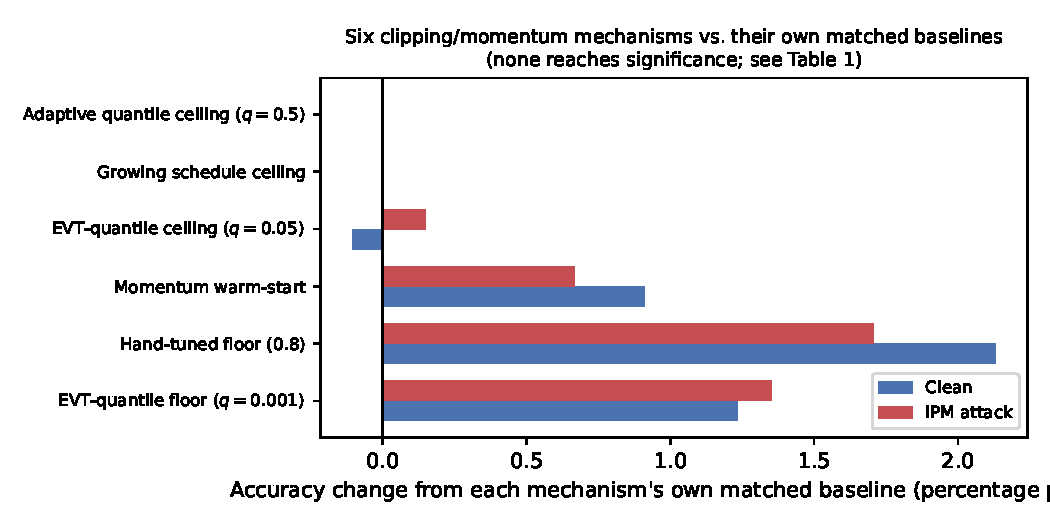
\includegraphics[width=0.85\linewidth]{figures/fig_audit_delta.pdf}
\caption{The six clipping/momentum mechanisms from Table~\ref{tab:audit-summary},
each shown as its accuracy change from its \emph{own} correctly seed-matched
baseline (the $n{=}3$ and $n{=}10$ audit cells use different baseline samples,
so a single shared baseline bar would visually overstate or understate some of
these deltas). The two ceiling mechanisms with $n{=}10$ or $n{=}3$ exact-match
results sit at zero by construction; the two floor mechanisms and momentum
warm-start all move in the same direction, the floor mechanisms by more.}
\label{fig:audit-delta}
\end{figure}

No mechanism that adjusts clipping or momentum dynamics, tested six independent
ways with up to $n{=}10$ paired seeds, significantly recovers CIFAR-10 accuracy
under Byz-Clip21-SGD2M's published protocol.

\section{What Actually Explains the Gap}
\label{sec:resolution}

If none of the algorithm's own tunable mechanisms explain the collapse, the
remaining candidate is that the protocol never gave the architecture a realistic
opportunity to learn CIFAR-10 features at all: $T{=}80$ rounds, one local SGD
step per round, batch size 32, no augmentation, no normalization, features
learned from raw pixels from a random initialization, under a Byzantine-robust
and DP-capable protocol simultaneously. We test this directly, using only
standard, non-novel machinery, and report the result as a resolution of the
confound rather than as a new algorithm.

\paragraph{Pretrained, frozen backbone.} We reserve 5{,}000 of CIFAR-10's 50{,}000
training images (10\%, fixed seed) as a public pretraining split, strictly
disjoint from the 45{,}000-image client pool used for the federated phase. A
backbone is trained centrally (never federated-averaged, so \texttt{BatchNorm}'s
running-buffer aggregation problem, Section~\ref{sec:norm}, does not apply) on
this split, then frozen; only a lightweight two-layer FC head is federated-trained
on the resulting cached features, using the identical Byz-Clip21-SGD2M harness
otherwise unchanged. A first backbone (the architecture from
Section~\ref{sec:setup}, no augmentation, 15 epochs) already recovers
substantially: clean baseline (fixed $\tau$, no floor, no extra local steps) rises
from 17.13\%$\,\pm\,$3.15\% to 32.79\%$\,\pm\,$3.01\% ($n{=}10$). A second,
deeper backbone (three conv blocks, \texttt{BatchNorm}, standard CIFAR-10
augmentation -- random crop and horizontal flip, applied only during this
central, non-federated pretraining step -- 40 epochs) raises the baseline
further, to 54.23\%$\,\pm\,$2.45\%.

\begin{figure}[t]
\centering
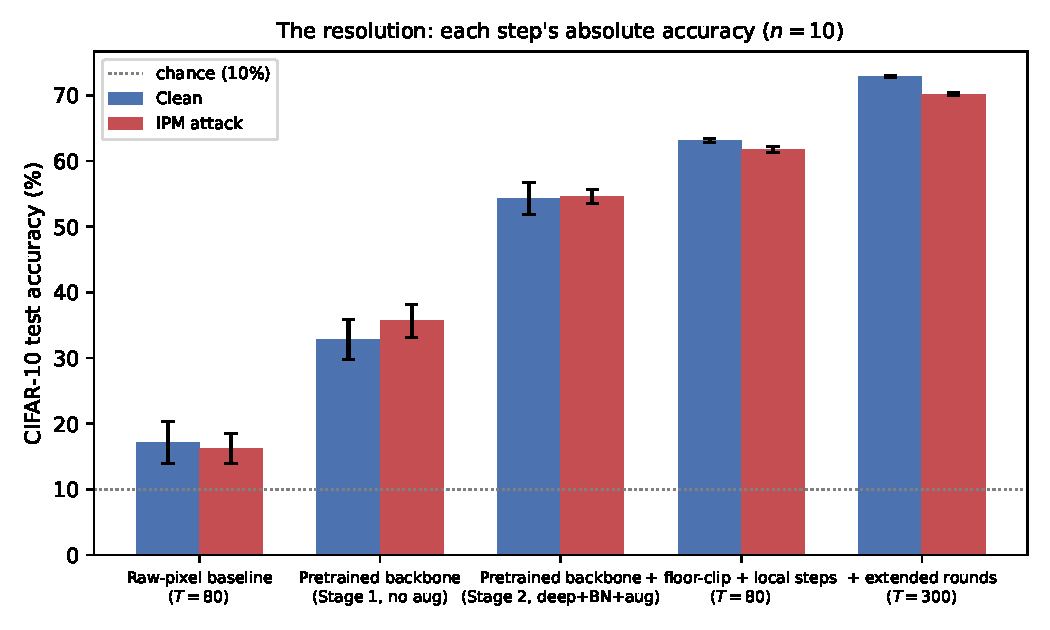
\includegraphics[width=0.9\linewidth]{figures/fig_resolution_absolute.pdf}
\caption{Absolute CIFAR-10 accuracy through the resolution's progression
(Section~\ref{sec:resolution}), $n{=}10$ per bar. Each step is a genuinely
different training regime rather than a matched-seed ablation of one algorithm,
so absolute accuracy -- not a delta from a shared baseline, cf.\
Figure~\ref{fig:audit-delta} -- is the appropriate comparison here.}
\label{fig:resolution-absolute}
\end{figure}

\paragraph{Stacking the one positive audit mechanism and local computation.}
Combining the second backbone with the floor-clipping mechanism from
Section~\ref{sec:floor} (floor $=0.8$) and multiple local SGD steps per round
(5 steps, local learning rate 0.01 -- the one rate independently found stable
for this architecture in Section~\ref{sec:lr}'s single-worker check -- converted
to a pseudo-gradient following \citet{reddi2021adaptive}), at the unchanged
$T{=}80$, $\gamma{=}0.1$: clean accuracy reaches 63.12\%$\,\pm\,$0.36\%
($n{=}10$, Wilcoxon $p{=}0.00195$ against the pretrained-but-untricked baseline
above -- every one of 10 seeds improves), and IPM-attacked accuracy reaches
61.75\%$\,\pm\,$0.40\% ($p{=}0.00195$). The gap between clean and
Byzantine-attacked accuracy at this configuration is 1.4 percentage points.

\paragraph{Disentangling floor-clip from local steps.} The configuration above
stacks two mechanisms -- floor-clip (Section~\ref{sec:floor}) and 5 local SGD
steps -- and Section~\ref{sec:floor} found this same floor mechanism, applied
alone on raw pixels, non-significant (+2.1pp clean / +1.7pp ipm, $n{=}10$).
This raises the question directly: on the pretrained backbone, is the
9-percentage-point combo gain actually driven by local computation, with
floor-clip contributing little, or the reverse? We isolate each mechanism on
the same Stage 2 backbone features, $T{=}80$, $n{=}3$ (the first 3 seeds of the
baseline and combo above, for a like-for-like comparison at matched $n$):
floor-clip alone (floor $=0.8$, local steps left at 1) moves clean accuracy
from 53.59\%$\,\pm\,$2.41\% to 60.94\%$\,\pm\,$0.70\% (+7.34pp) and IPM from
53.96\%$\,\pm\,$1.22\% to 59.61\%$\,\pm\,$0.61\% (+5.65pp); local steps alone (5
steps, floor disabled, i.e.\ the plain $\tau{=}1.0$ ceiling only) moves clean
accuracy to 55.39\%$\,\pm\,$1.76\% (+1.80pp) and IPM to 55.86\%$\,\pm\,$0.75\%
(+1.90pp). The two deltas sum to within 0.1--0.2 percentage points of the full
combo's own delta at this matched $n{=}3$ (+9.23pp clean, +7.43pp ipm) -- the
two mechanisms compose roughly additively, with no detectable synergy or
antagonism at this sample size. Floor-clip, not local computation, does the
majority of the work: roughly 80\% of the clean-condition gain and 76\% of the
IPM-condition gain. This is the opposite of what Section~\ref{sec:floor}'s
raw-pixel result would suggest in isolation -- the same mechanism (floor
$=0.8$) that was non-significant on raw pixels has a roughly 3.5$\times$
larger effect once applied to pretrained-backbone features. We do not have a
confirmed mechanistic explanation for this interaction and did not investigate
further; a plausible post-hoc reading is that floor-clip's benefit depends on
the diffs it rescales already carrying informative signal, which raw-pixel
gradients early in training may not -- but this is a reading, not a tested
claim. As with every other $n{=}3$ result in this paper, a paired Wilcoxon test
at this sample size cannot reach $p<0.25$ regardless of effect size, so these
numbers are effect-size evidence, not significance evidence; the direction
(floor $\gg$ local-steps, roughly additive) is nonetheless consistent across
all 3 seeds in both conditions (\texttt{scripts/cifar10\_ablation\_disentangle.py}).

\paragraph{Extended round budget.} The $T{=}80$ combined result's own accuracy
trace was still climbing at the final checkpoint (0.5865 $\to$ 0.5994 $\to$
0.6140 $\to$ 0.6275 across its last four evaluation points), so we extend to
$T{=}300$ -- an explicitly disclosed departure from both this paper's own
$T{=}80$ audit protocol and FedProto's $T{=}110$ CIFAR-10 convention
(Section~\ref{sec:related}), not blended silently into the $T{=}80$ comparison.
At $T{=}300$, $n{=}10$: clean accuracy reaches 72.88\%$\,\pm\,$0.14\%, IPM
reaches 70.17\%$\,\pm\,$0.20\% -- a further $\sim$10-percentage-point gain from
round budget alone, at unchanged $\gamma{=}0.1$.

\paragraph{Recommended configuration.} Of every configuration tested in this
paper, \textbf{pretrained backbone (Stage 2) + floor-clip (0.8) + 5 local steps
+ $\gamma{=}0.1$ + $T{=}300$} is the one we recommend as the paper's headline
resolution result: 72.88\%$\,\pm\,$0.14\% clean, 70.17\%$\,\pm\,$0.20\% IPM,
$n{=}10$, stable across every seed. The $T{=}80$ number
(63.12\%/61.75\%) above is the matched-audit-budget variant of the same
configuration, reported for direct comparability with Section~\ref{sec:audit};
it is not a worse alternative, only a smaller round budget. Everything in the
next paragraph is exploratory hyperparameter search reported for completeness
and transparency -- it is \emph{not} part of the recommended configuration and
should not be conflated with it.

\paragraph{Exploratory: does retuning $\gamma$ help further? (not part of the
recommended configuration).} The pretrained head's feature-gradient scale
differs from raw-pixel gradients and $\gamma{=}0.1$ was never independently
retuned for it. A sweep at $T{=}80$ found $\gamma{=}0.1$ itself under-tuned
there ($\gamma{=}0.3$ pilot, $n{=}3$: 70.06\%$\,\pm\,$0.32\% clean,
68.61\%$\,\pm\,$0.11\% ipm, versus 62.83\%/61.39\% at $\gamma{=}0.1$), with
$\gamma \geq 0.4$ destabilizing sharply (seed-to-seed range widening from 0.7
percentage points at $\gamma{=}0.3$ to roughly 16 percentage points at
$\gamma{=}0.4$, $\gamma{=}0.5$ collapsing outright on one seed to 27.09\%).
Combining $\gamma{=}0.3$ with the recommended $T{=}300$ ($n{=}10$), rather than
compounding the two improvements, reveals a striking asymmetry: the clean
condition destabilizes badly (34.92\%$\,\pm\,$11.46\%, individual seeds ranging
19.15\%--58.04\%, far below the recommended configuration's stable 72.88\%),
while the IPM-attacked condition stays tight and slightly exceeds the
recommended configuration's result (72.64\%$\,\pm\,$0.22\%, versus 70.17\%). We
do not have a confirmed explanation and did not investigate further; the shape
is consistent with the robust aggregator's trimming incidentally damping the
instability this higher learning rate causes when actual outlying (Byzantine)
contributions give it something to trim, while providing no such damping when
there is nothing unusual to discard. \textbf{This is why $\gamma{=}0.1$, not
$\gamma{=}0.3$, is the recommended configuration above}: it is the only one
tested that is simultaneously stable and strong on both conditions. We report
the $\gamma{=}0.3$/$T{=}300$ result to avoid quietly dropping a finding that
complicates, rather than supports, the otherwise-tidy "just retune $\gamma$"
narrative this paragraph started with -- not because it changes our
recommendation.

\paragraph{Robustness check: does the recommended configuration hold at larger
scale?} Everything above uses 20 clients (16.7\% Byzantine under attack),
matching Section~\ref{sec:setup}'s convention. At double the client count (40
clients, 32 regular + 8 Byzantine, same ratio; $T{=}80$ for compute reasons,
$n{=}3$ pilot), clean accuracy reaches 62.93\%$\,\pm\,$0.40\% and IPM-attacked
accuracy reaches 60.77\%$\,\pm\,$0.59\%, both within roughly 1 percentage point
of the 20-client $T{=}80$ numbers (63.12\%/61.75\%). This is consistent with
the recovery not being an artifact of the specific client count tested, though
a single doubled-scale, $n{=}3$ pilot bounds, rather than eliminates, the scale
caveat in Section~\ref{sec:limitations}.

\paragraph{Two conditions the recommended configuration does NOT hold under:
DP noise and non-IID data.} Everything reported above uses $\epsilon{=}\mathrm{None}$
(no DP noise) and IID partitioning. Both are real limits on what "the gap is
resolved" means, and we report them here rather than let the abstract's
Byzantine-robustness claim be read as broader than it is.

\emph{DP noise.} Reintroducing DP noise at the source paper's own privacy
budgets ($\epsilon \in \{18, 8\}$, $T{=}80$, $n{=}3$) collapses the recovery
almost entirely: clean accuracy falls to 19.19\%$\,\pm\,$1.62\% at
$\epsilon{=}18$ and 14.33\%$\,\pm\,$0.60\% at $\epsilon{=}8$ (versus 63.12\%
with no DP noise); IPM-attacked accuracy falls to 10.11\%$\,\pm\,$1.23\% at
$\epsilon{=}18$ and 10.13\%$\,\pm\,$1.97\% at $\epsilon{=}8$ -- within
0.11 and 0.13 percentage points of the 10\% chance floor respectively, and
well within one standard deviation of it at \emph{both} privacy levels
tested. As with every other $n{=}3$ result in this paper, we do not run a
formal test against chance at this sample size and report only the
descriptive proximity; the qualitative pattern (accuracy near chance under
attack once DP noise is active) is nonetheless unambiguous by eye across all
3 seeds at both $\epsilon$ values. Byz-Clip21-SGD2M's whole point is joint Byzantine-robustness
\emph{and} differential privacy; this configuration resolves the CIFAR-10 gap
only in the no-DP regime, and under real DP noise plus a Byzantine attacker
simultaneously, the collapse this paper set out to explain reappears in full.

\emph{Non-IID data.} Under Dirichlet label skew ($\alpha{=}0.5$, $T{=}80$,
$n{=}3$), the clean condition holds up well (baseline 53.36\%$\,\pm\,$1.67\%,
combo 63.18\%$\,\pm\,$0.24\%, matching the IID combo's 63.12\% almost exactly),
but Byzantine robustness does not: IPM-attacked accuracy is
38.24\%$\,\pm\,$5.50\% for the combo (baseline 31.58\%$\,\pm\,$6.04\%) --
still an improvement over the non-IID baseline, but a roughly 23-percentage-point
drop from the IID combo's 61.75\%, and both non-IID cells carry much higher
seed-to-seed variance (5--6 percentage points, versus well under 1pp IID).

Neither finding is a failure of the audit's own claims -- the six ruled-out
clipping/momentum mechanisms and the floor mechanism's modest signal are
unaffected by round budget, client count, DP noise, or partitioning, since
those audits were never claimed to depend on the resolution succeeding. It is
a real limit on how much weight the resolution (Section~\ref{sec:resolution})
alone can bear: it resolves the gap in the no-DP, IID setting tested, and
provides no evidence that it resolves the algorithm's actual target setting
(DP and Byzantine robustness, jointly, under realistic heterogeneity).

\begin{figure}[t]
\centering
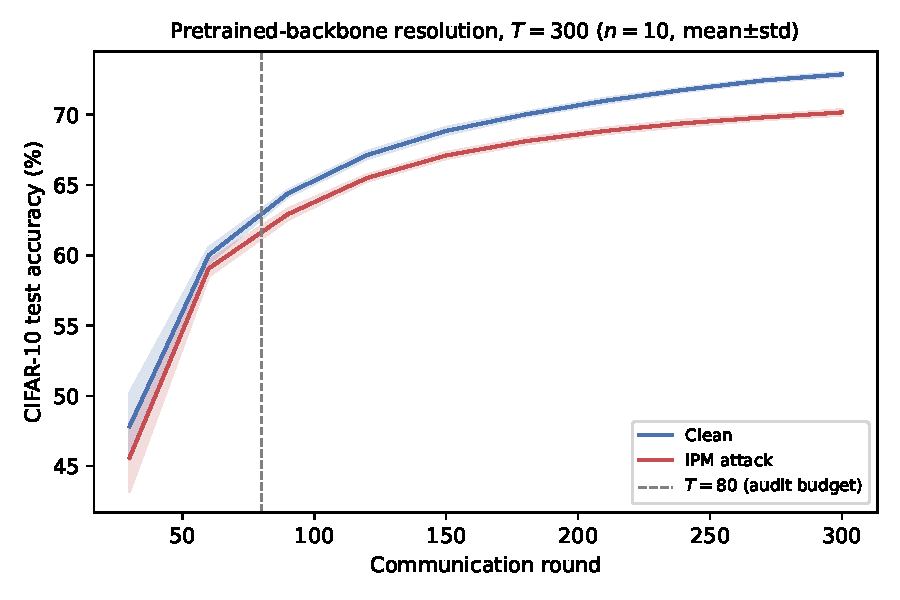
\includegraphics[width=0.8\linewidth]{figures/fig_round_trace.pdf}
\caption{Accuracy vs.\ communication round for the $\gamma{=}0.1$, $T{=}300$
combined configuration, $n{=}10$, mean $\pm$ one standard deviation shaded. The
dashed line marks $T{=}80$, this paper's own audit round budget: both curves
are still climbing well past it, which is why we report $T{=}300$ as an
explicitly disclosed extended-budget result rather than stopping at $T{=}80$.}
\label{fig:round-trace}
\end{figure}

\paragraph{What this does and does not show.} This is transfer learning and
FedAvg's local-computation mechanism \citep{mcmahan2017fedavg}, applied for the
first time to this specific algorithm's evaluation -- not a new algorithm, and we
make no claim that it is. We report it because it is the only
mechanism in this paper, out of eight tested, that produces a large, unambiguous,
statistically decisive effect, and because the size of that effect is itself
informative: a gap this large, closed by standard tools untried in the original
protocol, is stronger evidence that the original collapse was a protocol
artifact than any of the six ruled-out mechanisms in Section~\ref{sec:audit}
could provide on their own. It also does not show that this resolution
generalizes beyond the no-DP, IID conditions it was tested under: the DP-noise
and non-IID checks above found the recovery collapses almost entirely under
real DP noise and loses most of its Byzantine robustness under label skew.
The evidence that the \emph{original collapse} was a protocol artifact stands
on its own; the evidence that \emph{this specific fix} solves the algorithm's
actual joint DP-and-Byzantine-robustness target does not.

\section{Attempting a Comparison with FedProto}
\label{sec:fedproto-attempt}

Section~\ref{sec:related} explains why FedProto \citep{tan2022fedproto} is not a
like-for-like baseline for Byz-Clip21-SGD2M (different threat model, different
aggregated object -- prototypes, not gradients or weights -- different preferred
metric). We attempted a scoped, clean-condition comparison anyway, on the
reasoning that a compute-feasible approximation of FedProto's own protocol
(Table~\ref{tab:fedproto-diagnostic}'s header) would still be informative. It
surfaced a failure mode independent of, but structurally identical to, this
paper's central subject, and we report that failure mode rather than a
misleading accuracy number obtained around it.

\paragraph{What happened.} We implemented FedProto from its published equations
(prototype computation, the classification-plus-prototype-alignment loss, and
weighted-mean server aggregation; not from the original authors' code, which we
did not consult) and ran it under the closest protocol to FedProto's own paper
(20 clients, batch size 8, $\lambda{=}0.1$, IID CIFAR-10) that this project's CPU
budget could support. FedProto specifies one full local epoch per round
($\sim$312 steps/client/round at CIFAR-10's $\sim$2500 images/client); at 20
clients and the paper's own $T{=}110$, that is $\sim$686{,}000 forward/backward
passes, well beyond what the rest of this project's pilot-scale compute has
used. We first tried a reduced local-step count (5/round). The result was mean
client accuracy pinned at \emph{exactly} 10.0\% (chance) for the entire run.

\paragraph{Diagnosing it, rather than reporting it at face value.} A collapsed,
exactly-chance accuracy this clean is itself a signature worth checking rather
than accepting -- exactly the standard this paper has applied to every other
result in it. Tracking the global prototypes' own norm across rounds (rather
than only the downstream accuracy) showed why: the prototype-alignment loss has
a trivial degenerate minimizer -- collapsing every class's embedding toward the
same point drives the regularization term to zero without requiring correct
classification -- and with too little classification-loss gradient per round to
counteract it, training collapses into exactly that minimizer. Inspecting
individual client models directly confirmed this: every one of three inspected
models predicted a single fixed class for all 10{,}000 test images (classes 7,
2, and 2 respectively), the precise mechanism that produces an exact 10.0\%
on a class-balanced ten-way test set.

\begin{table}[t]
\centering\small
\begin{tabular}{lcc}
\toprule
Local steps/round & 3 clients & 20 clients \\
\midrule
5 & collapses (0.33 $\to$ 0.03, 15 rounds) & -- \\
15 & partial collapse (0.20, 15 rounds) & -- \\
25 & stable ($\approx$0.41, 15 rounds) & collapses (0.04, 15 rounds) \\
40 & stable ($\approx$0.42, 15 rounds) & -- \\
50 & -- & collapses (0.06, 15 rounds) \\
100 & stable ($\approx$0.34, 15 rounds) & collapses (0.05, 15 rounds) \\
\bottomrule
\end{tabular}
\caption{Mean global-prototype norm (a proxy for representation collapse: near
zero means every class's embedding has converged to the same point) as a
function of local computation per round and client count. The same local-step
budget that stabilizes training at 3 clients collapses it at 20 -- client count,
not only local computation, drives this failure mode, and even 100 steps/round
(40\% of a full local epoch at this data size) does not stabilize it at
FedProto's own 20-client convention.}
\label{tab:fedproto-diagnostic}
\end{table}

\paragraph{Why we stop here rather than force a number.} Table~\ref{tab:fedproto-diagnostic}
shows the failure is sensitive to both local computation \emph{and} client
count, and that the reduced budgets this project's compute can support at 20
clients do not avoid it -- closing the gap would require approaching FedProto's
own full-local-epoch budget, which we estimate at several hours of additional
CPU compute for a single seed/condition and did not run. Reporting an accuracy
number from a collapsed configuration, or quietly increasing local steps until
an arbitrary-looking number appeared, would be exactly the
kind of unexamined result this paper argues against accepting at face value in
Section~\ref{sec:audit}. We therefore report the diagnosed failure mode itself
as the finding.

\paragraph{Why this is not a wasted attempt.} This failure mode is, independently
of Byz-Clip21-SGD2M, a second demonstration of the paper's central point: an
accuracy collapse this clean (exactly at chance, not merely poor) is a signature
of an under-provisioned training budget, not necessarily a property of the
algorithm being evaluated. We did not have to look for a second example of this
-- it appeared during an attempt to build a comparison, in a completely
different algorithm (prototype aggregation, not gradient-based), under a
completely different mechanism (representation collapse under a regularizer's
degenerate minimizer, not gradient clipping or momentum dynamics). That two
unrelated algorithms both produce a clean, diagnosable, budget-driven collapse
under reduced compute is, if anything, stronger evidence for this paper's
general caution than either instance alone.

\section{The Growing-vs.-Bounded Clipping Tension}
\label{sec:tension}

Independent of Section~\ref{sec:clip}'s negative empirical results, the exercise
of building the tail-adaptive mechanisms surfaced a conceptual point we believe
has not been stated explicitly elsewhere. \citet{sun2024gradnorm}'s
convergence guarantee for heavy-tailed noise requires a clipping threshold that
\emph{grows without bound} as training proceeds ($h \propto
T^{2p/(3p-2)}$). Byz-Clip21-SGD2M's Byzantine-robustness guarantee, in common
with clipping-based robust aggregation generally, relies on $\tau$
\emph{bounding} the magnitude any single client's contribution can reach. A
threshold cannot simultaneously grow without bound and stay bounded: past
whatever point a heavy-tail-optimal schedule would place $\tau$, an adversary
can inject a contribution of arbitrary magnitude and the clipping mechanism no
longer constrains it. \textbf{To be precise about what this observation is and
is not: it identifies incompatible prescriptions between the two specific
analyses we checked (Section~\ref{sec:clip}), not a proven impossibility result
for any algorithm jointly achieving heavy-tail-optimal convergence and
Byzantine robustness} -- the full statement of that caveat follows below, and
we do not treat the observation as license to claim more than it establishes
anywhere else in this paper. Tying $\tau_t$ to an online estimate of the \emph{current}
robust scale (our EVT-quantile design, Section~\ref{sec:clip}) sidesteps this by
construction -- a stable scale estimate keeps $\tau$ bounded -- at the
acknowledged cost of not literally reproducing the moment-bound theorem's
asymptotic guarantee. We state this as a design consideration future work in
this specific intersection (heavy-tailed noise \emph{and} Byzantine robustness,
jointly) should account for, not as a theorem: we have not proven that no
schedule can satisfy both properties, only that the two most natural candidates
in the literature we checked make incompatible prescriptions.

\paragraph{What is proven and what is conjectured, stated plainly.} No result in
this section or Section~\ref{sec:clip} constitutes a convergence proof for any
tail-adaptive variant of Byz-Clip21-SGD2M. A full proof would need to combine (i)
\citeauthor{islamov2026byzclip}'s EF21 and Byzantine-robust-aggregation argument
for the $g_i/m_i/\mathrm{RAgg}$ recursion, (ii) a heavy-tailed high-probability
argument for the noise term inside that recursion adapted from a quantile-
rather than moment-based threshold, and (iii) a concentration argument for
$\hat\alpha_t/\hat\sigma_t$ being estimated online from a rolling window rather
than known constants. None of the three has been done, here or, to our
knowledge, elsewhere; we report the tension above as a design observation
motivating that combination, not as a claim that we have carried it out.

\section{Limitations}
\label{sec:limitations}

\paragraph{Scale.} All experiments run on CPU with small architectures (a
two-to-three-conv-layer CNN, a two-layer FC head) and pilot-scale compute
throughout. Section~\ref{sec:resolution}'s recommended configuration was
additionally checked at double the client count (40 vs.\ 20) and held within
about 1 percentage point of the 20-client numbers, which is some evidence
against the recovery being an artifact of that one client count -- but this is
a single doubled-scale, $n{=}3$ check, not a scaling study, and it says
nothing about whether the audit's five ruled-out mechanisms (Section~\ref{sec:audit},
tested only at 20 clients) would remain ruled out at production scale (larger
models, many more clients, GPU-scale training).

\paragraph{Sample sizes vary by mechanism, and we report this rather than
smoothing over it.} Only the adaptive-quantile ceiling remains at $n{=}3$, for
the principled reason given in Section~\ref{sec:clip}: it is a
mechanistically-proven no-op, so a larger sample would not change its
conclusion. Every other clipping/momentum mechanism -- learning-rate retuning,
GroupNorm, the growing-schedule ceiling (both conditions), the EVT-quantile
ceiling, momentum cold-start, and the two floor mechanisms -- now reaches the
full $n{=}10$ with paired significance testing, including the growing-schedule
ceiling's IPM condition, which an earlier draft of this audit left at $n{=}3$
after a background job computing it was killed mid-run; it has since been
completed and is consistent with the mechanistically-proven no-op status
established for its clean condition (Wilcoxon $p{=}0.688$, small
floating-point-scale deviations from baseline attributable to ordinary
non-determinism in multi-threaded CPU execution, not to the clipping mechanism
engaging). The DP-noise and non-IID checks, and the floor-clip/local-steps
disentangling ablation (all Section~\ref{sec:resolution}), are $n{=}3$ pilots,
the smallest-$n$ results in the paper to carry this much weight -- appropriate
for a first check of whether the recovery survives at all (it substantially
does not, for DP; substantially degrades, for non-IID Byzantine robustness) or
of which mechanism drives it (floor-clip contributes the large majority of the
combo's gain in both conditions, local steps a smaller minority), but not for
precise magnitudes, and a priority for scaling up before treating those
specific percentages as final. Table~\ref{tab:audit-summary} states the $n$
used for every reported number.

\paragraph{The multiple-comparison correction now covers every mechanism
tested at $n{=}10$.} Section~\ref{sec:setup} applies a Bonferroni correction to
a 21-test confirmatory family spanning every clipping/momentum/learning-rate/
normalization mechanism reaching $n{=}10$. Two tests survive: learning-rate
retuning at $\gamma{=}0.02$ and $\gamma{=}0.01$, both in the harmful direction.
The correction does not change any conclusion about whether a mechanism
\emph{beneficially} recovers accuracy -- none does, corrected or not -- but it
does confirm that the one significant departure from baseline in this entire
audit is robust to the strictest multiple-comparison bar applied anywhere in
this paper. The adaptive-quantile ceiling remains excluded from this family for
the reason given above (never rerun at $n{=}10$), not because a $p$-value would
be invalid for a proven no-op -- the growing-schedule ceiling, also a proven
no-op, is included precisely because it was rerun at $n{=}10$ and its
inclusion changes nothing.

\paragraph{The extended round budget is a real disclosure, not a footnote to
bury.} The $T{=}300$ result in Section~\ref{sec:resolution} uses roughly
$2.7\times$ FedProto's own CIFAR-10 round budget and $3.75\times$ this paper's
own $T{=}80$ audit protocol. We report both the matched-budget ($T{=}80$) and
extended-budget ($T{=}300$) numbers explicitly rather than only the larger,
more flattering one.

\paragraph{Not a completed comparison against FedProto or any other baseline
algorithm.} As stated in Section~\ref{sec:related}, we do not claim
Section~\ref{sec:resolution}'s pipeline outperforms FedProto or any other
specific method: the problems being solved, threat models, and evaluation
metrics differ. We did attempt a scoped clean-condition comparison
(Section~\ref{sec:fedproto-attempt}), but it surfaced a training-budget failure
mode rather than a completed, trustworthy accuracy number, and we report that
failure mode rather than a number obtained by forcing past it. No accuracy-level
comparison against FedProto has been executed under matched, non-collapsed
conditions in this paper.

\section{Broader Impact Statement}
\label{sec:broader-impact}

This paper is a methodological audit: it diagnoses why an existing algorithm's
published evaluation protocol under-performs, and identifies which of several
candidate explanations account for that gap. It introduces no new attack
capability -- the IPM, label-flip, and prototype-manipulation adversary models
used throughout (Section~\ref{sec:setup}, Section~\ref{sec:fedproto-attempt})
are all already published in the cited prior work, applied here for diagnosis,
not developed further. All experiments use MNIST \citep{lecun2010mnist} and
CIFAR-10 \citep{krizhevsky2009cifar}, long-standing public benchmark datasets
with no personally identifiable or sensitive content, no human-subjects
concerns, and no consent or licensing issues beyond their standard, widely-used
terms. We do not foresee a plausible path from this paper's findings -- about
evaluation-protocol confounds and a training-budget failure mode -- to a
harmful application or dual use, and accordingly see no risk that warrants
specific mitigation beyond what responsible disclosure of a Byzantine-robust
learning method's known failure modes already provides.

\section{Conclusion}
\label{sec:conclusion}

A CIFAR-10-scale accuracy collapse in a Byzantine-robust, differentially private
federated learning algorithm is not, in this case, explained by three
independently-constructed clipping-ceiling mechanisms (two mechanistically-proven
no-ops, confirmed with matched-seed, paired statistical tests; the third, an
extreme-value-theory variant not a proven no-op by construction, also reaching
$n{=}10$ and showing no significant effect), by learning-rate transfer or
missing normalization (both now tested at $n{=}10$: retuning the learning rate
downward is significantly \emph{worse}, robust to Bonferroni correction across
every mechanism audited in this paper, and normalization's one
uncorrected-significant cell does not survive that correction -- neither shows
a beneficial direction in any cell), or by momentum cold-start (a small,
non-significant effect at $n{=}10$). A fifth candidate, a missing clipping
floor, showed a small, consistent positive direction that never reached
significance ($p \geq 0.064$) even when its hand-tuned constant was replaced by
a measurement-driven one -- a real effect too modest to explain the gap on its
own, reported as such rather than rounded up. In the no-DP, IID setting
actually tested, the gap is instead substantially explained by standard
machinery absent from the original evaluation protocol: a pretrained, frozen
backbone, the same floor-clipping mechanism from the fifth candidate above,
and additional local computation per communication round -- a disentangling
ablation ($n{=}3$) attributes most of this combination's gain to floor-clipping
once applied on top of the backbone, not to local computation, the same
mechanism that was too modest to explain the gap in isolation on raw pixels.
We report this honestly as a non-novel resolution of that setting rather than
dress up as an invented algorithm. This resolution does not extend to the algorithm's
actual target setting: real DP noise collapses it almost entirely, and
non-IID data leaves the clean recovery intact while substantially eroding
Byzantine robustness -- we report both limits explicitly rather than let the
headline recovery numbers stand unqualified. An unplanned attempt to compare
against FedProto
\citep{tan2022fedproto} -- an unrelated, prototype-aggregating algorithm --
independently reproduced the same caution under reduced compute: an
exactly-chance collapse diagnosable to a training-budget artifact, not a
property of that algorithm either, which we report as a failure mode rather
than force into a misleading accuracy comparison. We hope the audit itself --
and the two design iterations in it that failed for a diagnosable reason and
were fixed or reported rather than hidden -- is useful to others evaluating
this class of algorithm on datasets harder than MNIST.

\bibliographystyle{tmlr}
\bibliography{main}

\end{document}
